%% Bookheader, Nov 8, 2020; July 18, 2022

\documentclass[11pt]{../Support/ourbook}
%% or for landscape, comment out line above and use this one:
%%\documentclass[landscape,11pt]{ourbook}

%% This will keep space from stretching around display math:

\makeatletter
\renewcommand\normalsize{%
   \@setfontsize\normalsize\@xipt{13.6}%
   \abovedisplayskip 11\p@  \@minus6\p@
   \abovedisplayshortskip \z@ 
   \belowdisplayshortskip 6.5\p@ \@minus3\p@
   \belowdisplayskip \abovedisplayskip
   \let\@listi\@listI}
\makeatother
\normalsize


\begin{document}

\tableofcontents
\graphicspath{{../../Chapters/exponents_review/en_US}}
\chapter{Exponents}

Let's quickly review exponents. Ancient scientists started coming up
with a lot of formulas that involved multiplying the same number
several times. For example, if they knew that a sphere was $r$
centimeters in radius, its volume in milliliters was

$$V = \frac{4}{3} \times \pi \times r \times r \times r$$

They did two things to make the notation less messy. First, they
decided that if two numbers were written next to each other, the
reader would assume that meant ``multiply them''. Second, they came
up with the exponent, a little number that was lifted off the
baseline of the text, that meant ``multiply it by itself''. For
example $5^3$ was the same as $5 \times 5 \times 5$.\index{exponents}

Now the formula for the volume of a sphere is written

$$V = \frac{4}{3} \pi r^3$$

Tidy, right? In an exponent expression like this, we say that $r$ is
\textit{the base} and $3$ is \textit{the exponent}.

\section{Identities for Exponents}

What about exponents of exponents?  What is $\left(5^3\right)^2$?

$$\left(5^3\right)^2 = (5 \times 5 \times 5)^2 = (5 \times 5 \times 5)(5 \times 5 \times 5) = 5^6$$

In general, for any $a$, $b$, and $c$:

$$\left(a^b\right)^c = a^{(bc)}$$

If you have $\left( 5^3 \right) \left(5^4 \right)$ that is just $5 \times 5 \times 5 \times 5 \times 5 \times 5 \times 5$ or $5^7$

The general rule is, for any $a$, $b$, and $c$

$$\left(a^b\right)\left(a^c\right) = a^{(b + c)}$$

Mathematicians \textit{love} this rule, so we keep extending the idea
of exponents to keep this rule true. For example, at some point,
someone asked ``What about $5^0$?'' According to the rule, $5^{2}$
must equal $5^{(2 + 0)}$ which must equal
$\left(5^2\right)\left(5^0\right)$.  Thus, $5^2$ must be 1. So
mathematicians declared ``Anything to the power of 0 is 1''.\index{exponents!zero}

We don't typically assume that $0^0 = 1$. It is just too
weird. So we say, that for any $a$ not equal to zero,

$$a^0 = 1$$

What about $5^{(-2)}$?  By our beloved rule, we know that
$\left(5^{-2}\right)\left(5^5\right)$ must be equal to $5^3$, right?
So $5^{-2}$ must be equal to $\frac{1}{5^2}$.\index{exponents!negative}

We say, for any $a$ not equal to zero and any $b$,

$$a^{-b} = \frac{1}{a^{b}}$$

This makes dividing one exponential expression by another (with the same base) easy:

$$\frac{a^b}{a^c} = a^{(b-c)}$$

We often say ``cancel out'' for this. Here I can ``cancel out'' $x^2$:

$$\frac{x^5}{x^2} = x^3$$

What about $5^{\frac{1}{3}}$? By the beloved rule, we know that $5^{\frac{1}{3}}5^{\frac{1}{3}}5^{\frac{1}{3}}$ must equal $5^1$. Thus $5^{\frac{1}{3}} = \sqrt[3]{5}$.\index{exponents!fractions}

We say, for any $a$ and $b$ not equal to zero and any $c$ greater than zero,

$$a^{\frac{b}{c}} = a^b \sqrt[c]{a}$$

Before you go on to the exercises, note that the beloved rule demands a common base.
\begin{itemize}
\item We can combine these: $\left(5^2\right)\left(5^4\right) = 5^6$
\item We cannot combine: $\left(5^2\right)\left(3^5\right)$
\end{itemize}

With that said, we note for any $a$,$b$, and $c$:

$$\left(ab\right)^c = \left(a^c\right) \left(b^c\right)$$

So, for example, if I were asked to simplify
$\left(3^4\right)\left(6^2\right)$, I would note that $6 = 2 \times
3$, so

$$\left(3^4\right)\left(6^2\right) = \left(3^4\right)\left(3^2\right)\left(2^2\right)  = \left(3^6\right)\left(2^2\right)$$


If these ideas are new to you (or maybe they have been forgotten),
watch the Khan Academy's \textbf{Intro to rational exponents} video at
\url{https://youtu.be/lZfXc4nHooo}.

%https://www.pinterest.com/pin/800796377464592621/

\graphicspath{{../../Chapters/exponential_decay/en_US}}
\chapter{Exponential Decay}

In a previous chapter, we saw that an investment of $P$ getting
compound interest with an annual interest rate of $r$, grows
exponentially. At the end of year $t$, your balance would be

$$P\left(1 + r\right)^t$$

Because $r$ is positive, this number grows as time passes. You get a
nice exponential growth curve that looks something like this:

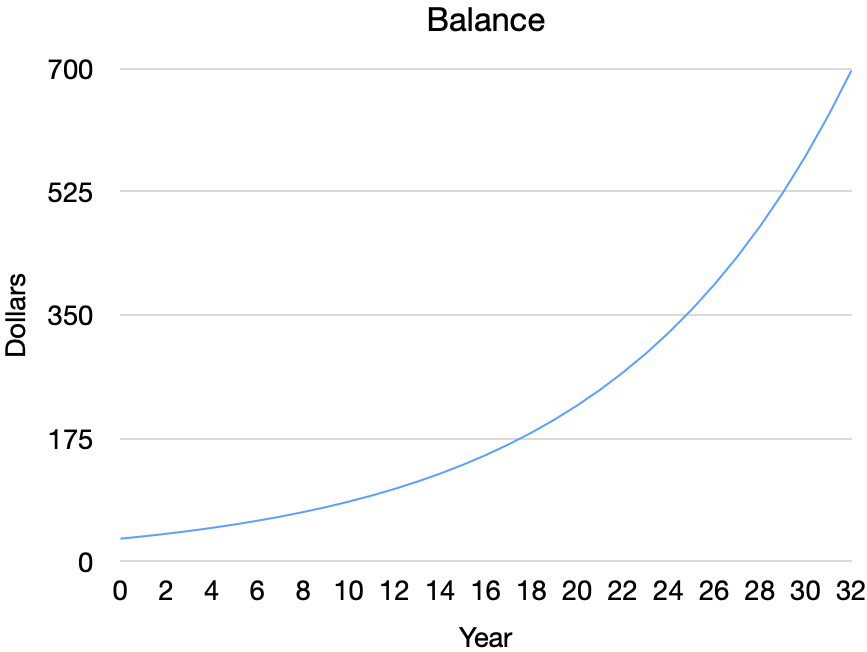
\includegraphics[width=0.7\textwidth]{exponential_growth.png}

This is \$30 invested with a 10\% annual interest rate. So, the formula
for the balance after $t$ years would be

$$(30)(1.1)^t$$

What if $r$ were negative? This would be \textit{exponential decay}.

\section{Radioactive Decay}

Until around 1970, there were companies making watches whose faces and
hands were coated with radioactive paint. The paint usually contained
radium. When a radium atom decays, it gives off some energy, loses two
protons and two neutrons, and becomes becomes a different element
(radon). Some of the energy given off is visible light. Thus, these
watches glow in the dark.\index{radioactive decay}

How many of the radium atoms in the paint decay each century? About 4.24\%.

Notice the quantity of atoms lost is proportional to the number of
atoms you have. This is exponential decay. If we assume that we start
with a million radium atoms, the number of atoms decreases over time like this:

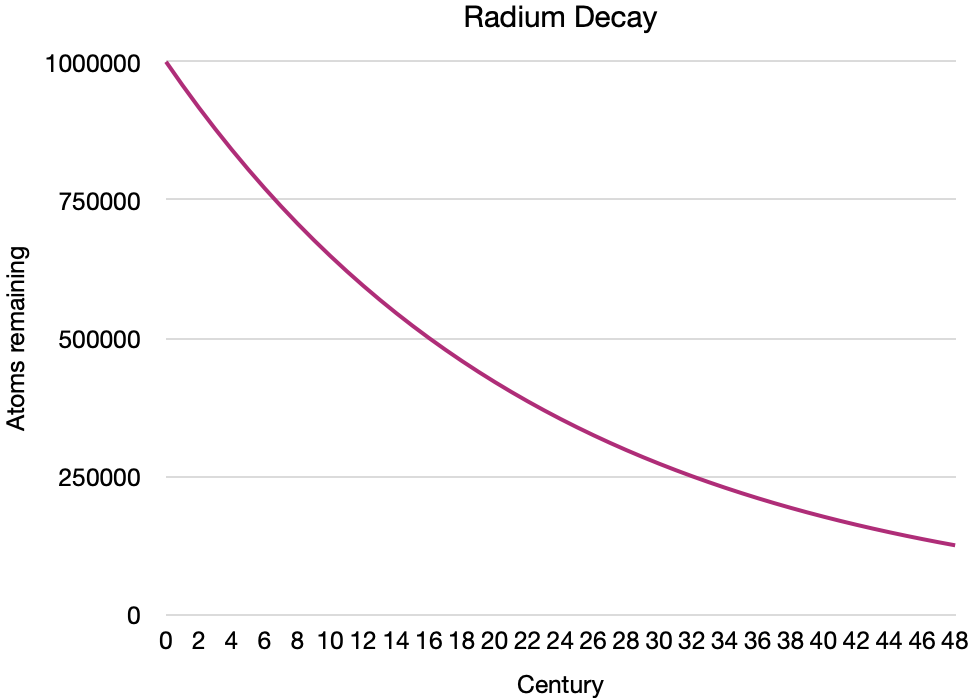
\includegraphics[width=0.7\textwidth]{radium_decay.png}
 
\begin{itemize}
\item We start with 1,000,000 atoms.
\item At 16 centuries, we have only 500,000 (half as many) left.
\item 16 centuries after that, we have only 250,000 (half again) left.
\item 16 centuries after that, we have only 125,000 (half again) left.
\end{itemize}

A nuclear chemist would say that radium has a \textit{half-life} of
1,600 years. Note that this means that if you bought a watch with
glowing hands in 1960, it will be glowing half as brightly in the year
3560.\index{half-life}

How do we calculate the amount of radium left at the end of century
$t$? If you start with $P$ atoms, at the end of the $t$-th century, you
will have

$$P\left(1 - 0.0424\right)^t$$

This is exponential decay.\index{exponential decay}
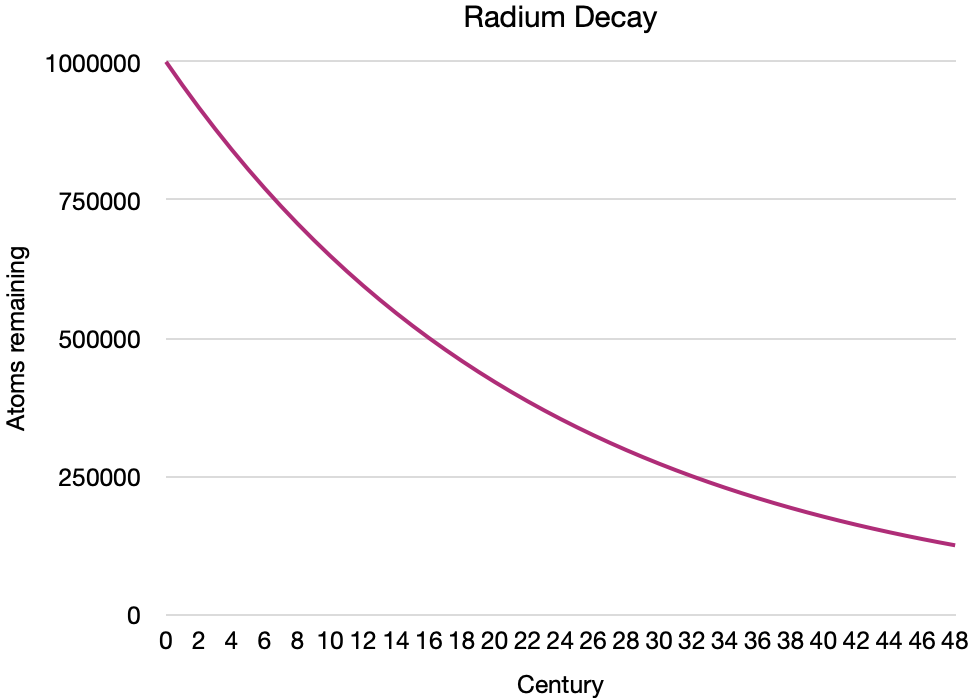
\includegraphics[width=0.7\textwidth]{radium_decay.png}

\section{Model Exponential Decay}

Let's say you get hired to run a company with 480,000
employees. Each year, $1/8$ of your employees leave the company for
one reason or another (retirement, quitting, etc.). For some reason, you never
hire any new employees.

Make a spreadsheet that indicates how many of the original 480,000
employees will still be around at the end of each year for the next 12. Next, make a
bar graph from that data.

\graphicspath{{../../Chapters/logs/en_US}}
\chapter{Logarithms}

After the world created exponents, it needed the opposite. We
could talk about the quantity $? = 2^3$, that is, ``What is the
product of 2 multiplied by itself three times?''  We needed some way
to talk about $2^? = 8$, that is, ``2 to the what is 8?'' This is why we
developed the logarithm.\index{logarithm} \index{log}

Here is an example:

$$\log_{2}8 = 3$$

In English, you would say, ``The logarithm base 2 of 8 is 3.''

The base (2, in this case) can be any positive number. The argument
(8, in this case) can also be any positive number.

Try this one: What is the logarithm base 2 of 1/16?

You know that $2^{-4} = \frac{1}{16}$, so $\log_{2} \frac{1}{16} = -4$.

\section{Logarithms in Python}

Most calculators have pretty limited logarithm capabilities, but
python has a nice \pyfunction{log} function that lets you specify both
the argument and the base. Start python, import the math module, and try taking a few logarithms:\index{log!in python}

\begin{Verbatim}
>>> import math
>>> math.log(8,2)
3.0
>>> math.log(1/16, 2)
-4.0
\end{Verbatim}

Let's say that a friend offers you 5\% interest per year on your
investment for as long as you want. You wonder, ``How many years
before my investment is 100 times as large?'' You can solve this problem with logarithms:

\begin{Verbatim}
>>> math.log(100, 1.05)
94.3872656381287
\end{Verbatim}

If you leave your investment with your friend for 94.4 years, the
investment will be worth 100 times what you put in.

\section{Logarithm Identities}

The logarithm is defined this way:\index{logarithm!identities}

$$\log_b a = c \iff b^c = a$$

Notice that the logarithm of 1 is always zero, and $\log_b b = 1$.

The logarithm of a product:

$$\log_b a c = \log_b a + \log_b c$$

This follows from the fact that $b^{a + c} = b^a b^c$. What about a quotient?

$$\log_b \frac{a}{c} = \log_b a - \log_b c$$

Exponents?

$$\log_b \left(a^c\right) = c \log_b a$$

Notice that because logs and exponents are the opposite of each other, they can cancel each other out:

$$b^{\log_b a} = a$$

and

$$\log_b \left(b^a\right) = a$$

\section{Changing Bases}

We mentioned that most calculators have pretty limited logarithm
capabilities. Most calculators don't allow you to specify what base
you want to work with. All scientific calculators have a button for
``log base 10''.  So, you need to know how to use that button to get
logarithms for other bases. Here is the change-of-base identity:\index{logarithm!change of base}

$$\log_b a = \frac {\log_c a}{\log_c b}$$

For example, if you wanted to find $\log_2 8$, you would ask the
calculator for $\log_{10} 8$, then divide that by $\log_{10} 2$.
You should get 3.

\section{Natural Logarithm}

When you learn about circles, you are told that the circumference of a
circle is about 3.141592653589793 times its diameter.  Because we use
this unwieldy number a lot, we give it a name: We say ``The
circumference of a circle is $\pi$ times its diameter.''

There is a second unwieldy number that we will eventually use a great deal in
solving problems. It is about 2.718281828459045 (but the digits
actually go on forever, just like $\pi$). We call this number $e$. (We are
not going to talk about why $e$ is special quite yet, but we will soon.)\index{e}\index{logarithm!natural}

Most calculators have a button labeled ``ln''. That is the
\textit{natural logarithm} button. It takes the log in base $e$.\index{ln}

Similarly, in python, if you don't specify a base, the logarithm is done in base $e$:

\begin{Verbatim}
>>> math.log(10)
2.302585092994046
>>> math.log(math.e)
1.0
\end{Verbatim}

\section{Logarithms in Spreadsheets}

Spreadsheets have three log functions:
\begin{itemize}
\item \pyfunction{LOG} takes both the argument and the base. \pyfunction{LOG(8,2)} returns 3.
\item \pyfunction{LOG10} takes just the argument and uses 10 as the base.
\item \pyfunction{LN} takes just the argument and uses $e$ as the base.
\end{itemize}

Here is a plot from a spreadsheet of a graph of $y = LOG(x, 2)$.

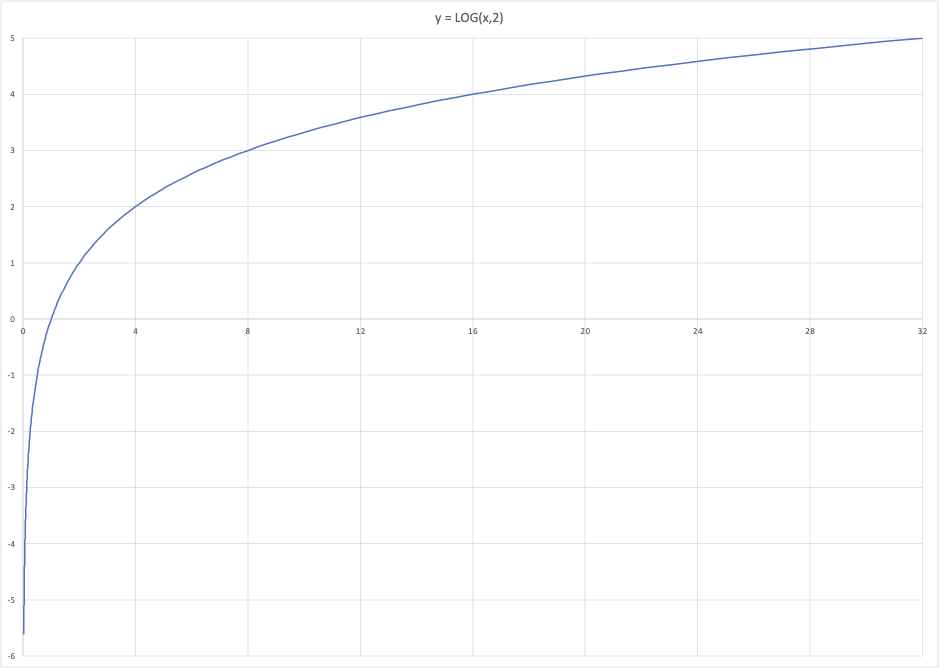
\includegraphics[width=0.8\textwidth]{log_graph.png}

Spreadsheets also have the function \pyfunction{EXP(x)}, which returns
$e^x$.  For example, \pyfunction{EXP(2)} returns 7.38905609893065.


%%%%%%%%%%%%%%%%%%%%%%%%%%%%%%%%%
%% Bookfooter.tex by Aaron Hillegass
%% Nov 8, 2020

\appendix

\chapter{Answers to Exercises}
\shipoutAnswer

\bibliography{references}

\printindex

\end{document}